\documentclass{article}

% Using / Including a package
\usepackage{amsmath}
\usepackage{graphicx}
\usepackage{subcaption}

% Adding a title page
\title{Title of my document}
\date{2013-09-01}
\author{John Doe}

\begin{document}
\maketitle
\pagenumbering{gobble}
\newpage
\pagenumbering{arabic}

% Summary

% A document has a preamble and document part
% The document environment must be defined
% Commands beginning with a backslash \, environments have a begin and end tag
% Useful settings for pagenumbering:
%   gobble - no numbers
%   arabic - arabic numbers
%   roman - roman numbers
\newpage


% Hierarchy of sectioning elements
\section{Section}
Hello World!
\subsection{Subsection}
Structuring a document is easy!
\subsubsection{Subsubsection}
More text.
\paragraph{Paragraph}
Some more text.
\subparagraph{Subparagraph}
Even more text.
\section{Another Section}

% Summary

% LaTeX uses the commands \section, \subsection and \subsubsection to define sections in your document
% The sections will have successive numbers and appear in the table of contents
% Paragraphs are not numbered and thus don't appear in the table of contents
\newpage


% Using math
\begin{equation}
f(x) = x^2
\end{equation}
\begin{equation*}
f(x) = x^2
\end{equation*}

% Summary

% Packages add new functions to LaTeX
% All packages must be included in the preamble
% Packages add features such as support for pictures, links and bibliography
\newpage


% Using inline math - embed formulas in your text
This formula $f(x) = x^2$ is an example.

% The equation and align environment
\begin{equation*}
1 + 2 = 3
\end{equation*}
\begin{equation*}
1 = 3 - 2
\end{equation*}
% Output
% 1 + 2 = 3
% 1 = 3 - 2

\begin{align*}
1 + 2 &= 3\\
1 &= 3 - 2
\end{align*}
% Output
% 1 + 2 = 3
%     1 = 3 - 2

% Fractions and more
\begin{align*}
    f(x) &= x^2\\
    g(x) &= \frac{1}{x}\\
    F(x) &= \int^a_b \frac{1}{3}x^3
\end{align*}

\begin{equation}
    \frac{1}{\sqrt{x}}
\end{equation}

% Matrix
\begin{equation*}
    \begin{matrix}
        1 & 0\\
        0 & 1
    \end{matrix}
\end{equation*}
% the matrices only work within math environments

% Brackets in math mode - Scaling
\begin{equation*}
    [
    \begin{matrix}
    1 & 0\\
    0 & 1
    \end{matrix}
    ]
\end{equation*}

\begin{equation*}
    \left[
    \begin{matrix}
        1 & 0\\
        0 & 1
    \end{matrix}
    \right]
\end{equation*}

\begin{equation*}
    \left(
        \frac{1}{\sqrt{x}}
    \right)
\end{equation*}

% Summary

% LaTeX is a powerful tool to typeset math
% Embed formulas in your text by surrounding them with dollar signs $
% The equation environment is used to typeset one formula
% The align environment will align formulas at the ampersand & symbol
% Single formulas must be seperated with two backslashes \\
% Use the matrix environment to typeset matrices
% Scale parentheses with \left( \right) automatically
% All mathematical expressions have a unique command with unique syntax
% Notable examples are:
%   \int^a_b for integral symbol
%   \frac{u}{v} for fractions
%   \sqrt{x} for square roots
% Characters for the greek alphabet and other mathematical symbols such as \lambda
\newpage


% Captioned images / figures in LaTeX
\begin{figure}
    
\includegraphics[width=\linewidth]{NewEngineeringDkBlue.png}
    \caption{Logo}
    \label{fig:logo1}
\end{figure}
Figure \ref{fig:logo1} shows a logo.

% Image positioning / setting the float
\begin{figure}[h!]
    
\includegraphics[width=\linewidth]{NewEngineeringDkBlue.png}
    \caption{Logo}
    \label{fig:logo1}
\end{figure}
Figure \ref{fig:logo1} shows a logo.
% h (here) - same location
% t (top) - top of page
% b (bottom) - bottom of page
% p (page) - on an extra page
% ! (override) - will force the specified location

% Multiple images / subfigures in LaTeX
\begin{figure}[h!]
    \centering
    \begin{subfigure}[b]{0.4\linewidth}
        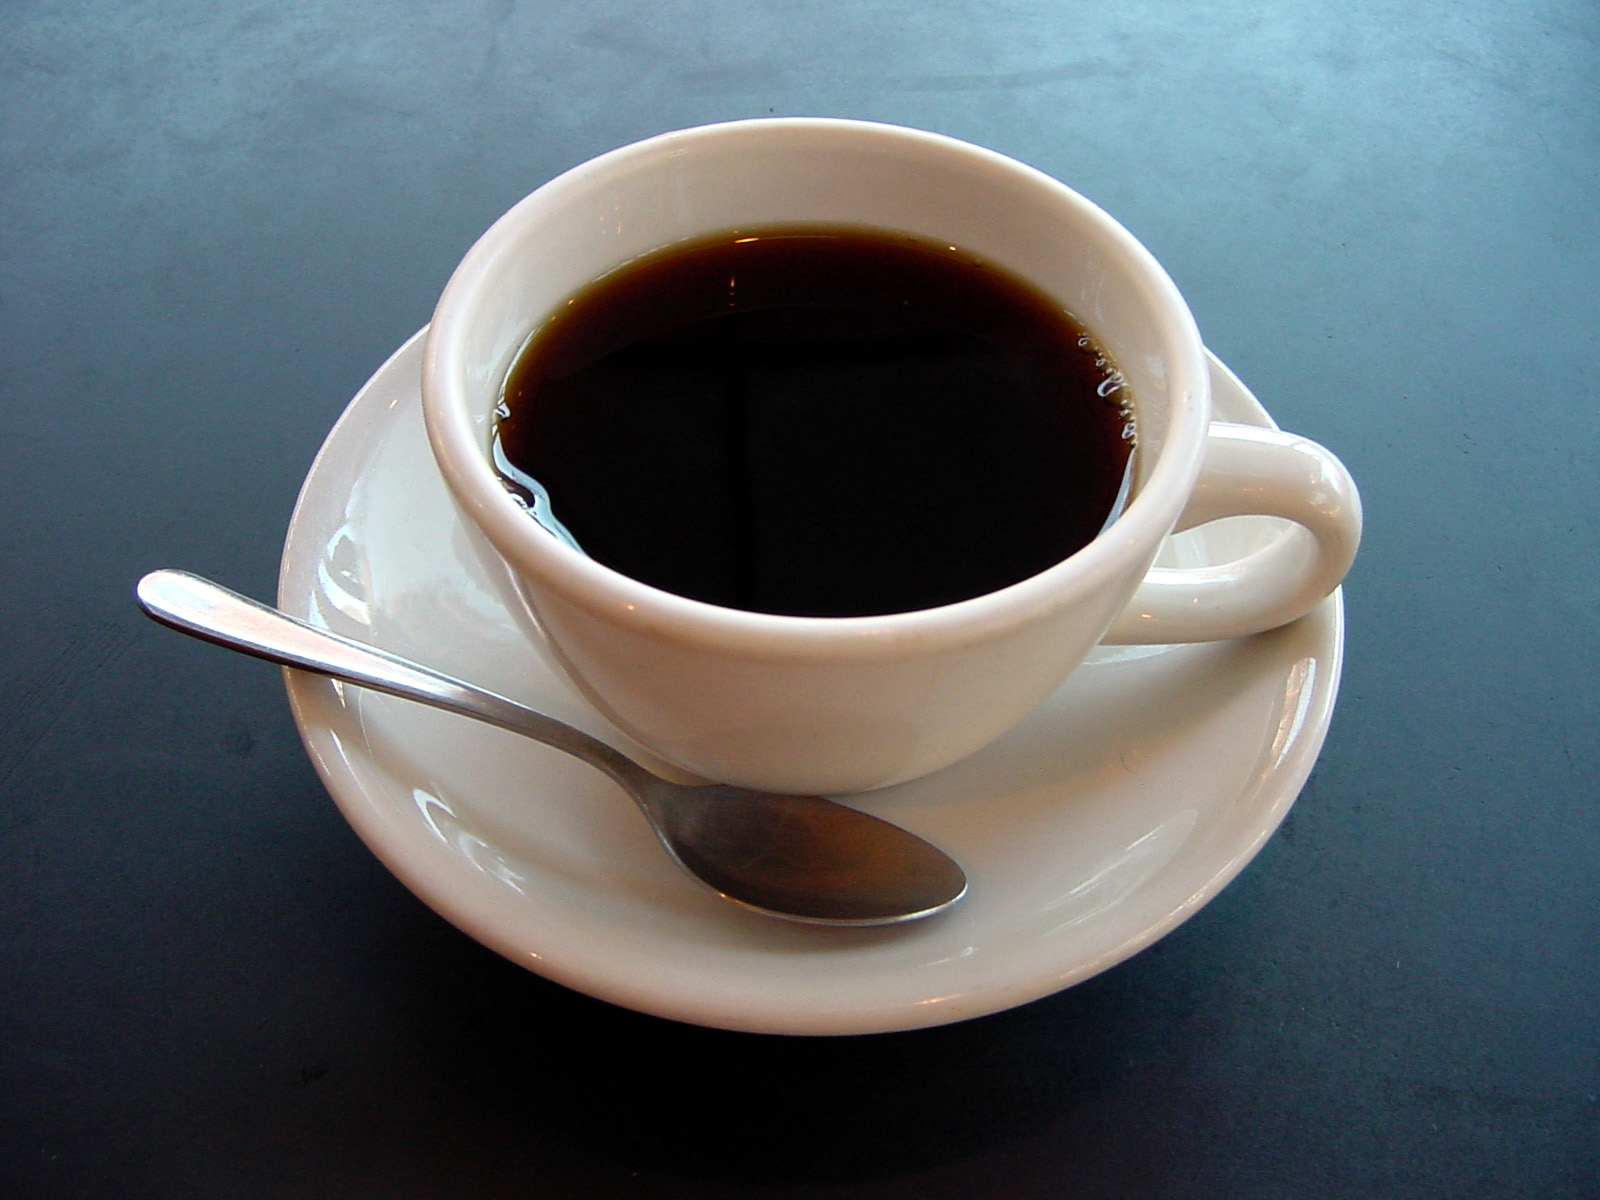
\includegraphics[width=\linewidth]{coffee.jpg}
        \caption{Coffee.}
    \end{subfigure}
    \begin{subfigure}[b]{0.4\linewidth}
        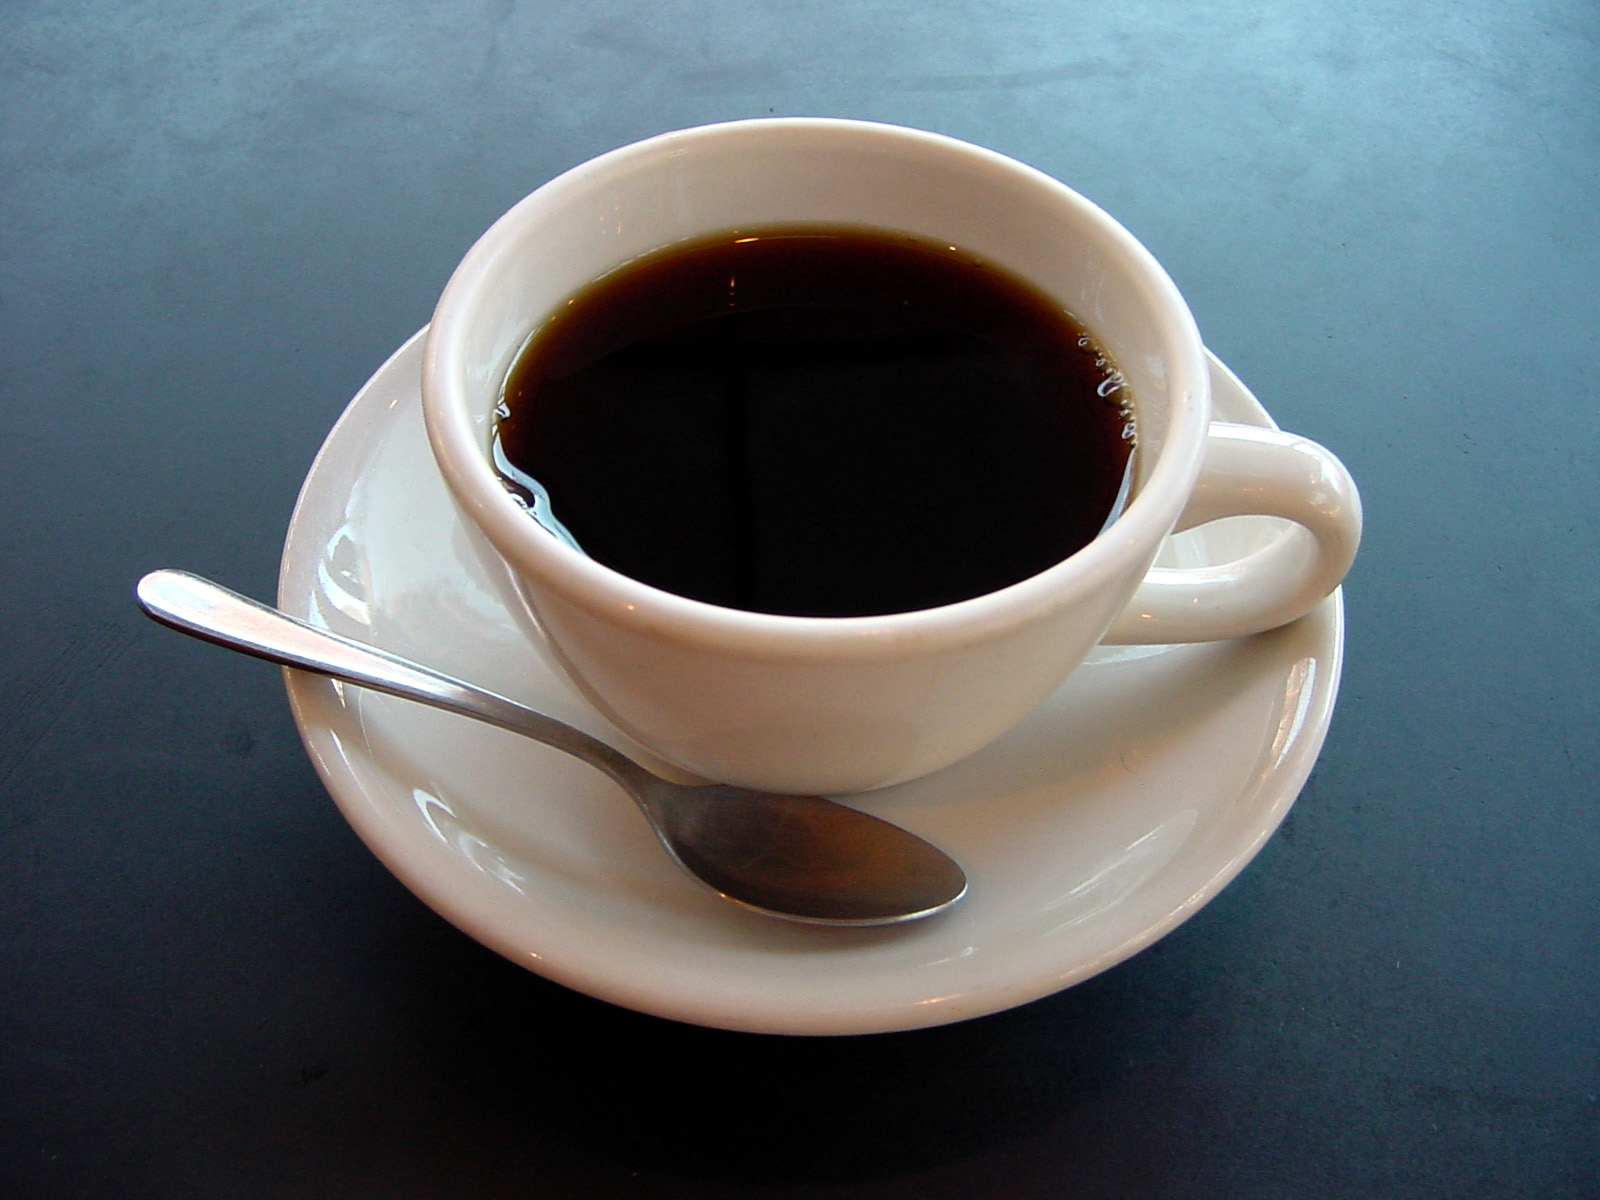
\includegraphics[width=\linewidth]{coffee.jpg}
        \caption{More coffee.}
    \end{subfigure}
    \caption{The same cup of coffee. Two times.}
    \label{fig:coffee}
  \end{figure}

\begin{figure}[h!]
    \centering
    \begin{subfigure}[b]{0.2\linewidth}
        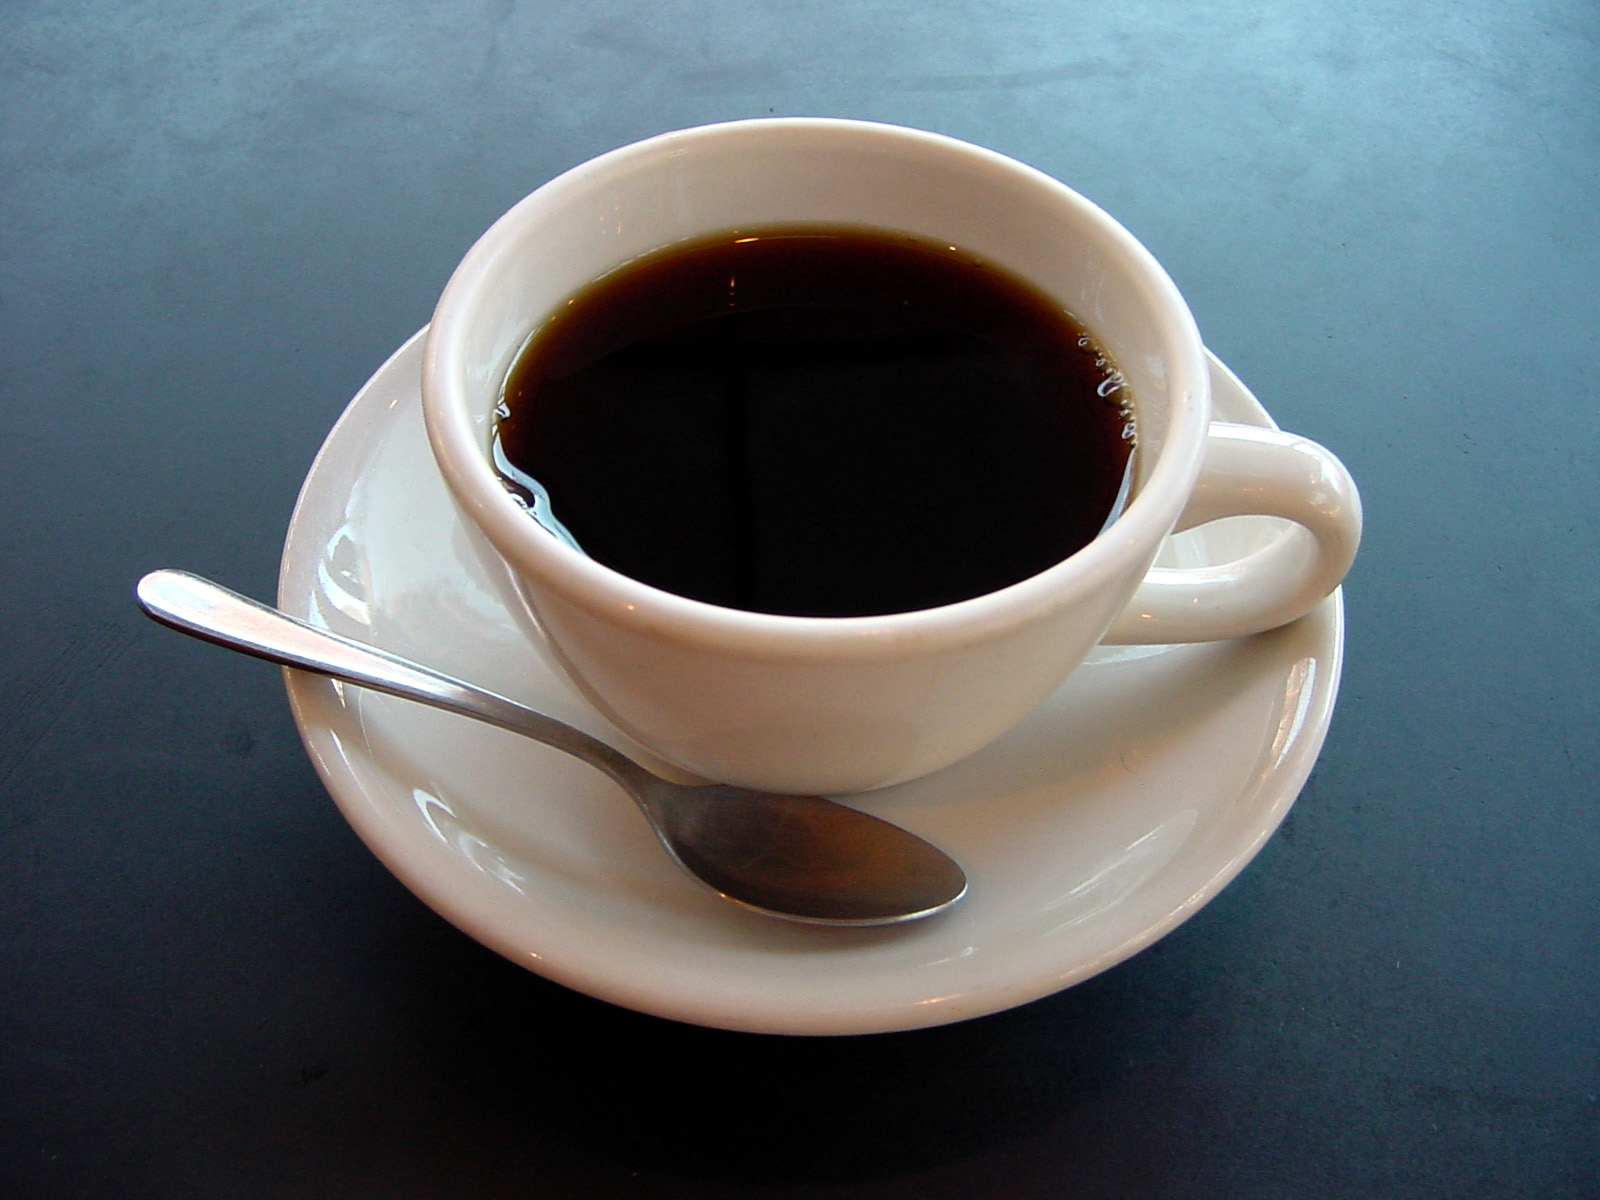
\includegraphics[width=\linewidth]{coffee.jpg}
        \caption{Coffee.}
    \end{subfigure}
    \begin{subfigure}[b]{0.2\linewidth}
        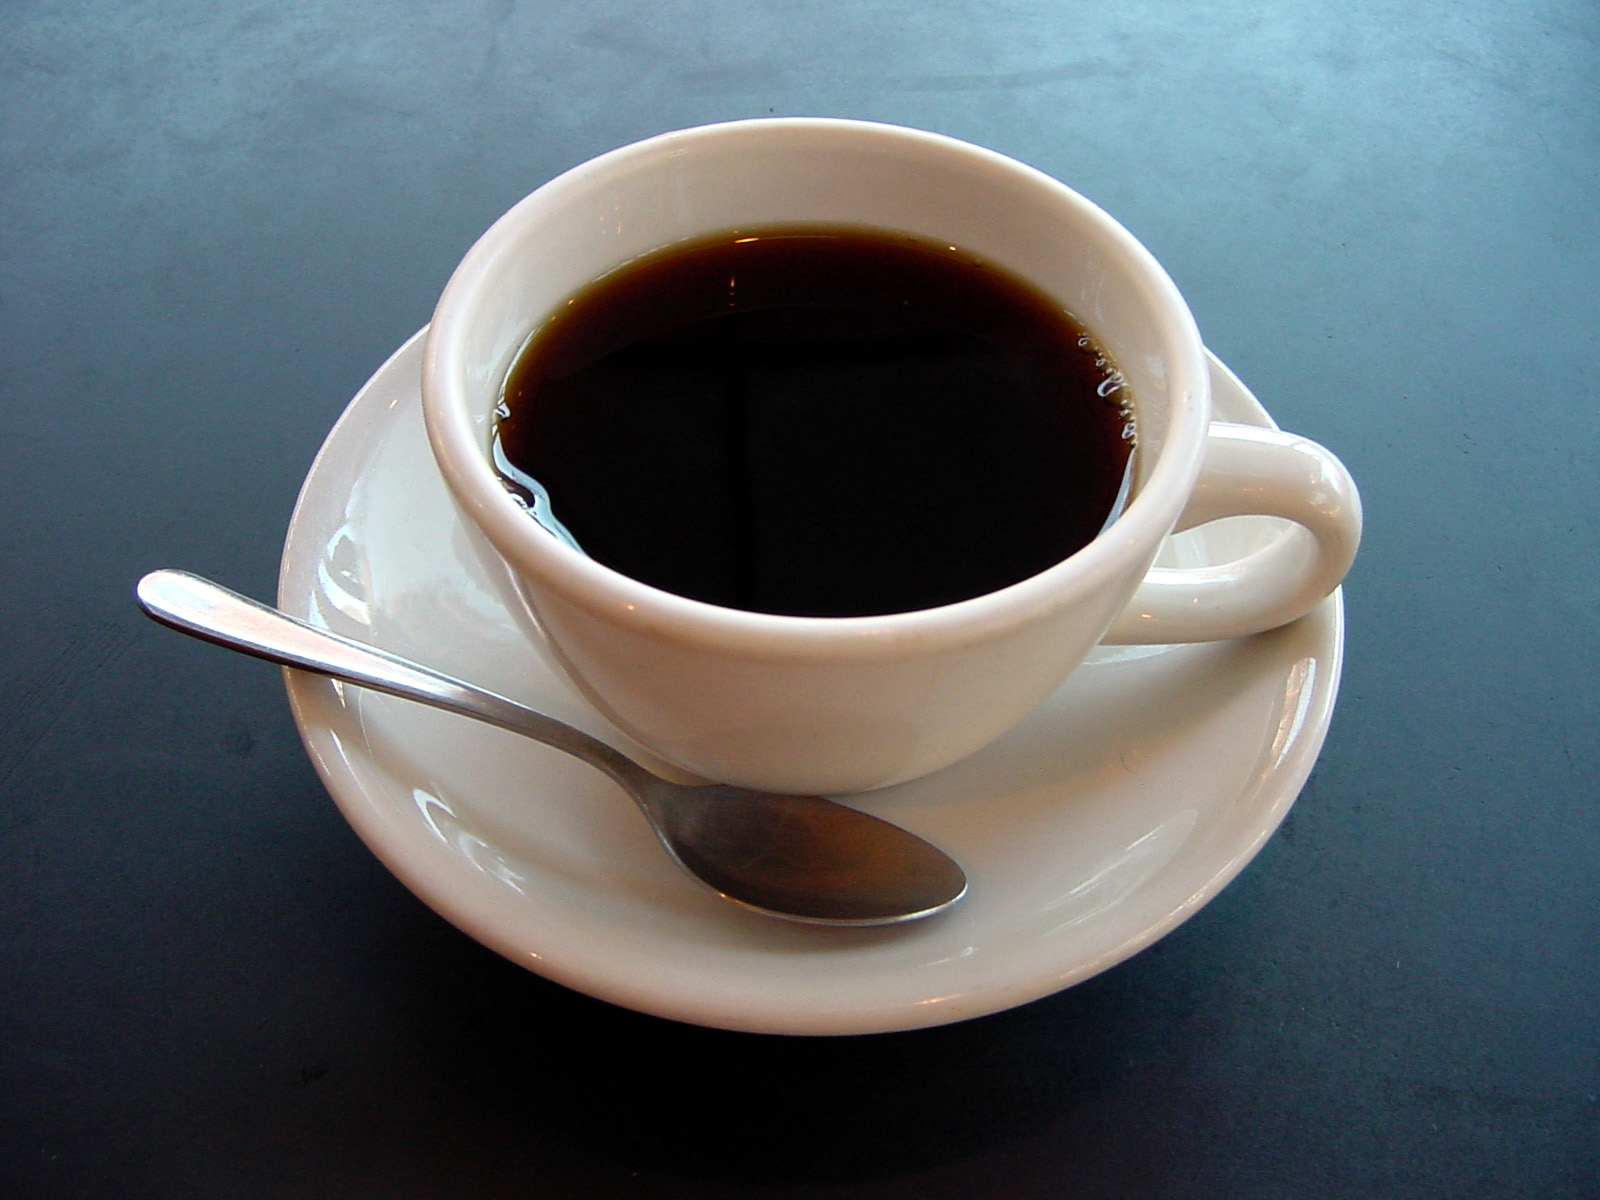
\includegraphics[width=\linewidth]{coffee.jpg}
        \caption{More coffee.}
    \end{subfigure}
    \begin{subfigure}[b]{0.2\linewidth}
        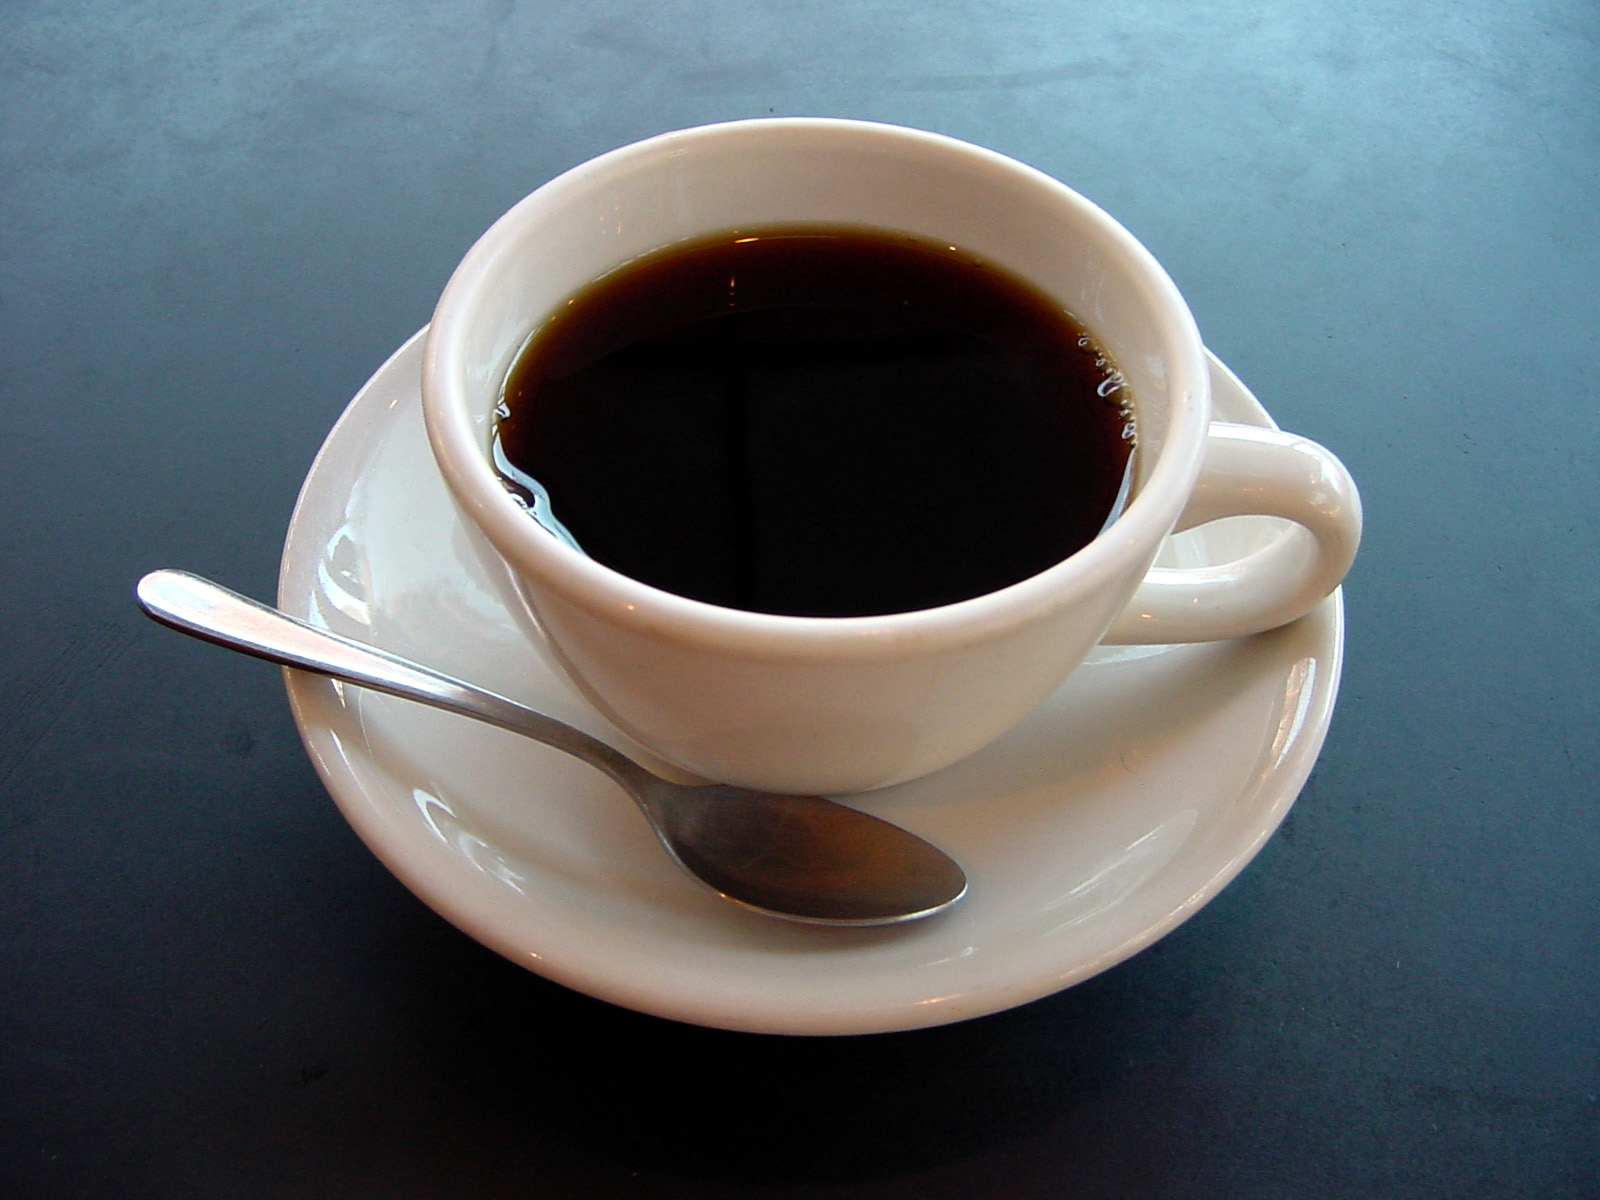
\includegraphics[width=\linewidth]{coffee.jpg}
        \caption{Tasty coffee.}
    \end{subfigure}
    \begin{subfigure}[b]{0.5\linewidth}
        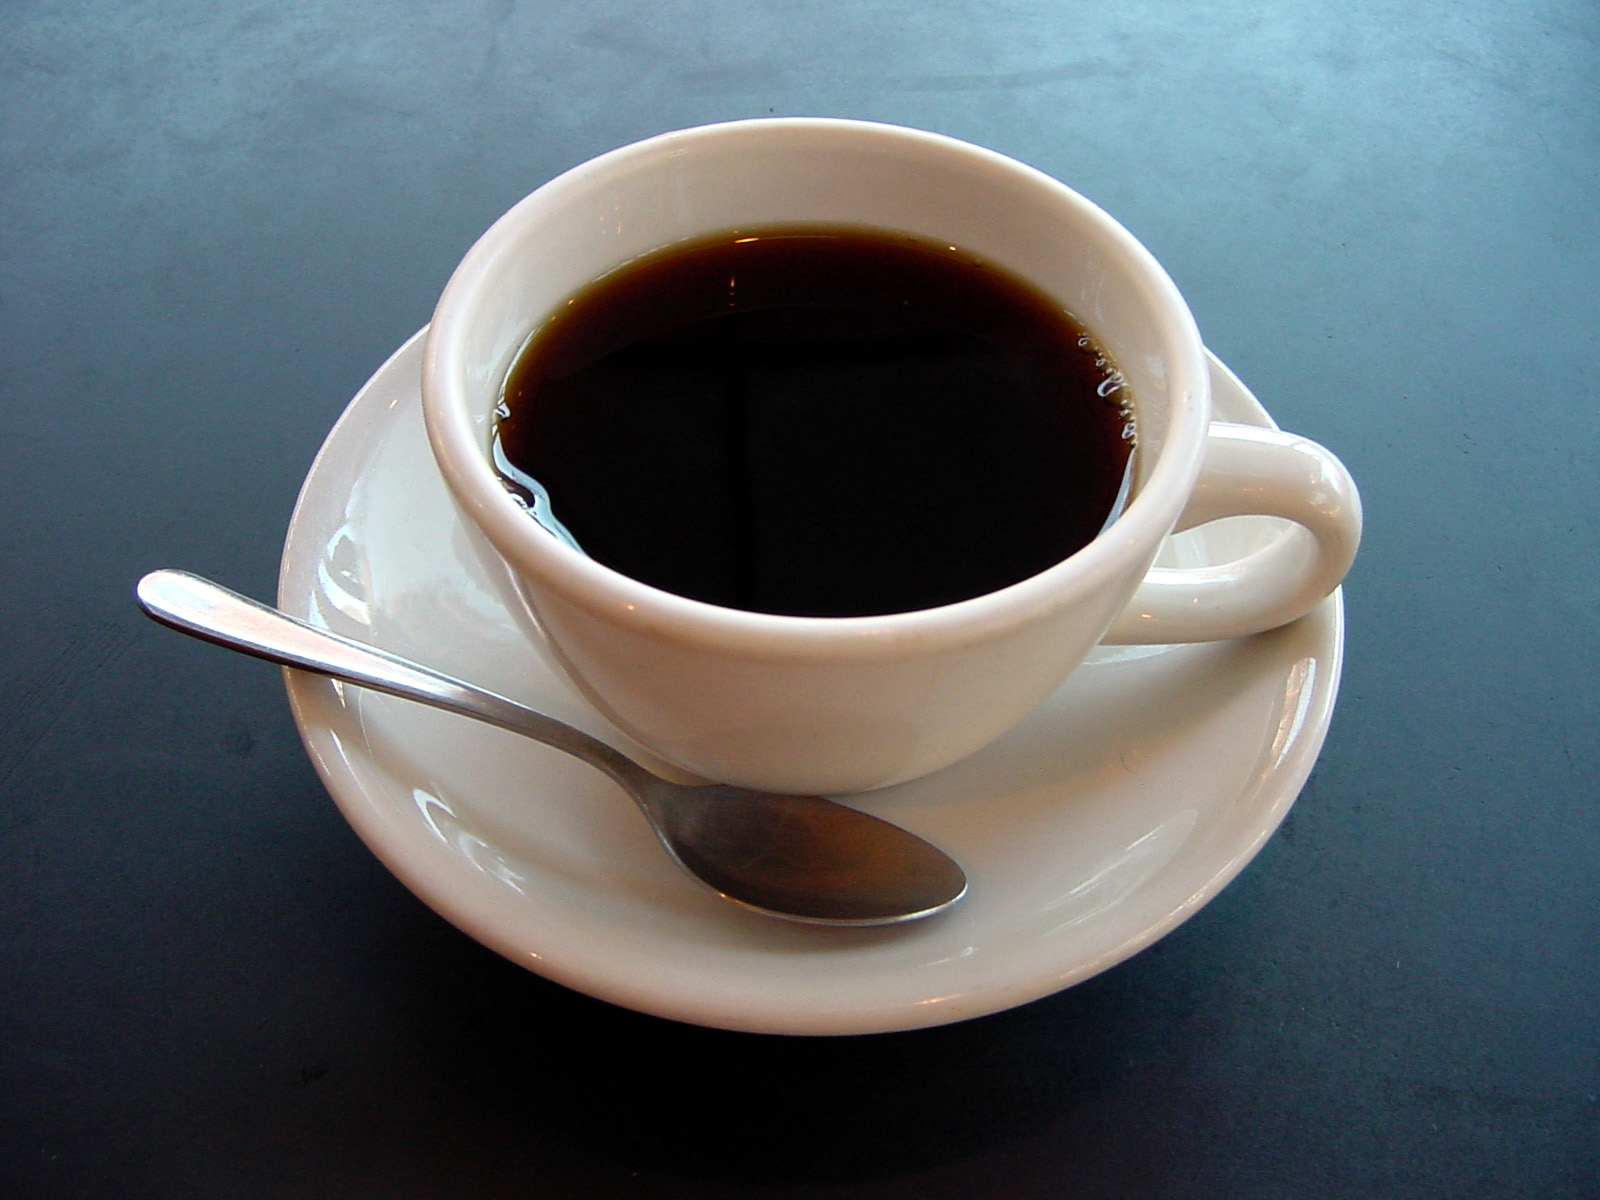
\includegraphics[width=\linewidth]{coffee.jpg}
        \caption{Too much coffee.}
    \end{subfigure}
    \caption{The same cup of coffee. Multiple times.}
    \label{fig:coffee3}
\end{figure}

% Summary

% Use the graphicx package and figure environment to embed pictures
% Pictures will be numbered automatically
% Change the width of your image by using \includegraphics[width=\linewidth]{}
% Refer to pictures in your document by setting a \label and using the \ref tag
% Set the position of your image by adding a float option such as [h!]
% If you want to show multiple figures next to each other, use the subcaption package and the subfigure environment
\newpage




\end{document}




